\documentclass[aspectratio=169]{beamer}
\usepackage{basileabeam}

% Notes:
%\pgfpagesuselayout{2 on 1}[a4paper,border shrink=5mm]
%\setbeamertemplate{note page}[plain]
%\setbeameroption{show notes on second screen=bottom}

\title              {Multithreaded Web Server}

\author             {Rahel Kempf, Ephraim Siegfried}
% \email              {author@email.com}
\institute          {Operating Systems, University of Basel}

\date               {3.5.2024}

\ulogo        		{Template/header}
\ulistelement    	{Template/listelement}

\graphicspath{{Figures/}}

% Options:
\totalNoSlidesDisabled % To turn off the total number of slides in the footer. Comment this if you want the total number of slides in the footer

\headerSectionsDisabled % Comment this if you want a fancy header containing your sections.


\begin{document}

\begin{frame}[t,plain]
\titlepage
\end{frame}

\note{Notes can help you to remember important information. Turn on the notes option.}

\section{Section 1}	% You can also have slides prior to the first section or work entirely without sections.

\begin{frame}[c]{Problem Statement}
\begin{columns}[c]
    \column{.55\textwidth}
            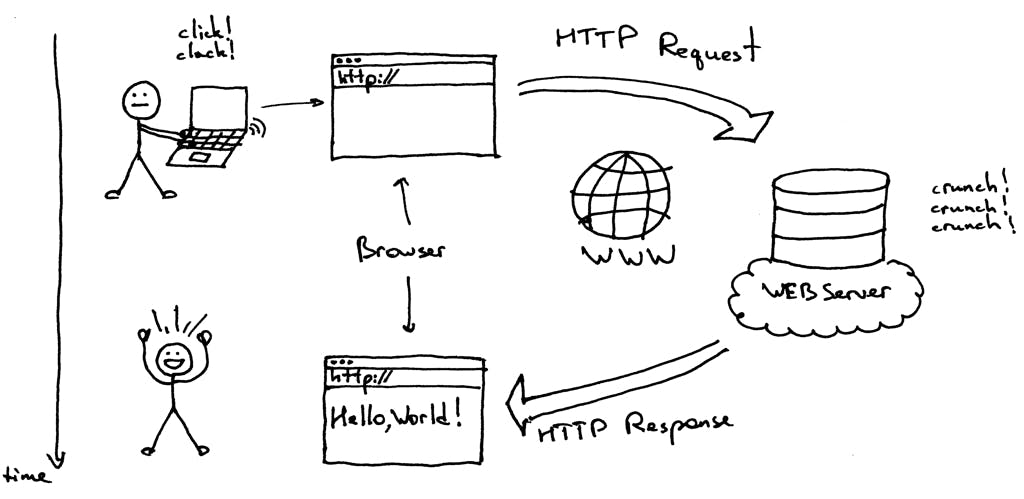
\includegraphics[width=\textwidth]{webserver-comic.jpg}
    \column{.45\textwidth}
   We visit web pages all the time and want to understand the underlying processes. Therefore we want to build our own web server.
\end{columns}
\end{frame}

\note{Notes can help you to remember important information. Turn on the notes option.}

\begin{frame}[c]{Proposed solution}
  A multithreaded web server with the following properties:
  \begin{itemize}
 \item Process HTTP requests
    \item Multiple clients can connect
    \item Simple database management / concurrent access to resources 
    \item Error handling: returning correct server errors
    \item Log web traffic
    \item Handle multiple domains and resources
    \item Hopefully: Websocket support
  \end{itemize}
\end{frame}

\note{Notes can help you to remember important information. Turn on the notes option.}

\begin{frame}[c]{Preliminary Time Plan}
  \centering
  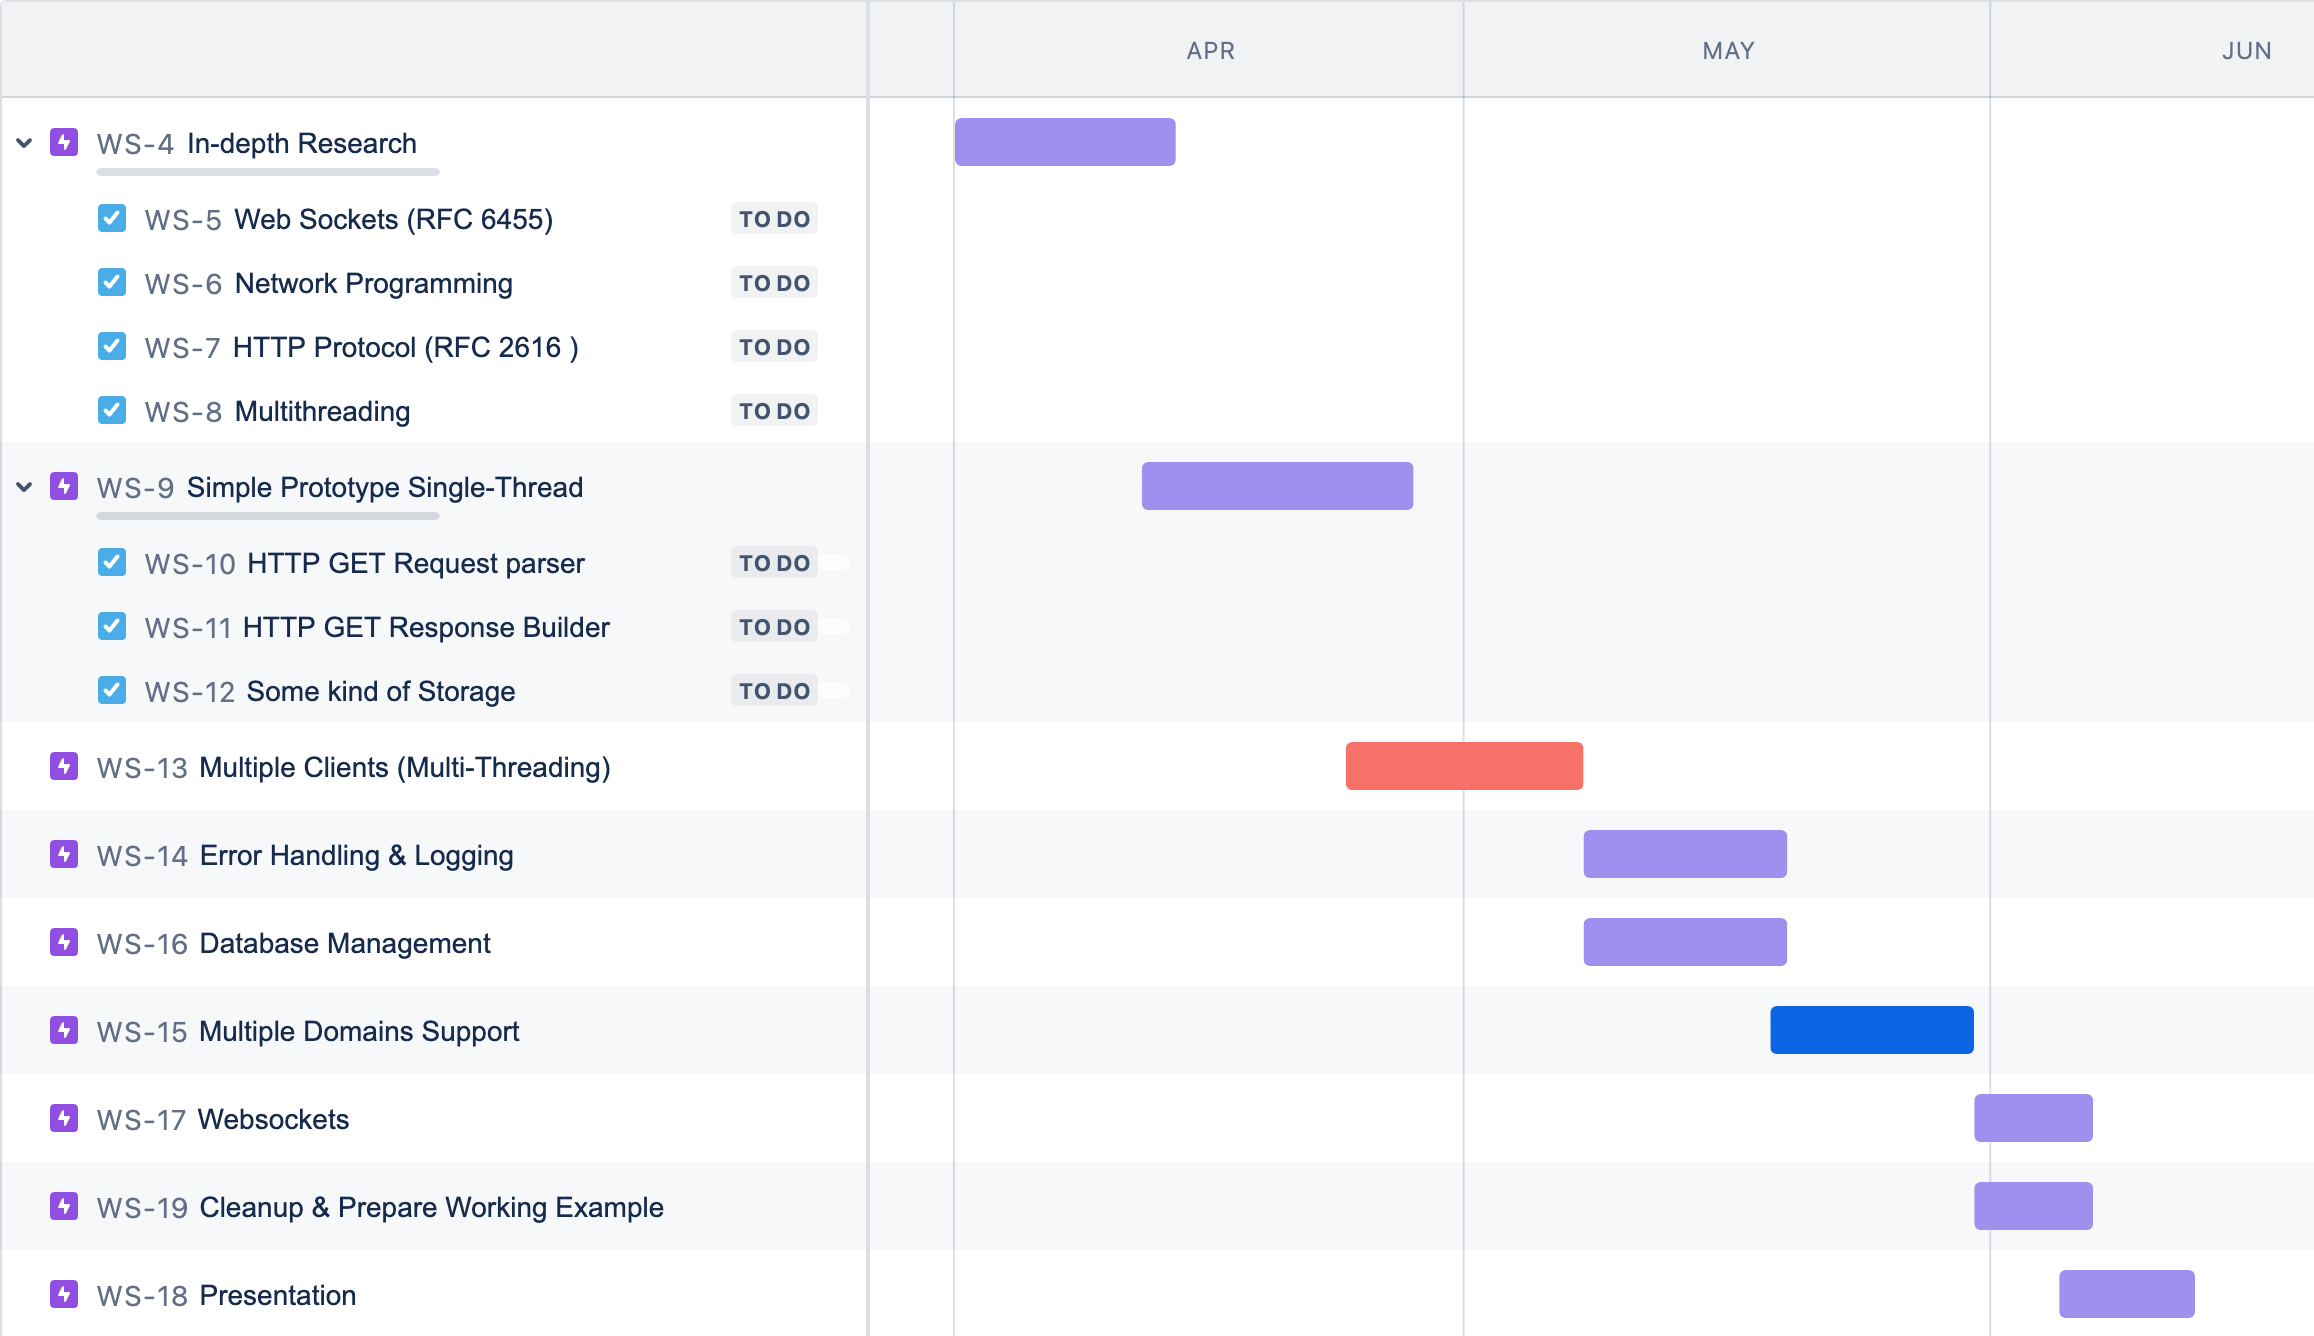
\includegraphics[width=0.8\textwidth]{gantt_chart.png}
\end{frame}

\note{Notes can help you to remember important information. Turn on the notes option.}

\section{Section 2}


\begin{frame}[t,plain]
  \lastpage{{\usebeamerfont{title} Questions?}}
\end{frame}

\end{document}

